\section{Diffraction}
L'optique géométrique ne suffit pas ! En regardant un réverbère la nuit à
travers le rideau d'une fenêtre, on voit autour du point lumineux central une
croix, éventuellement colorée, dont les bras sont perpendiculaires aux fils de
la toile du rideau. Lors de son passage à travers les petits trous du tissu, la
lumière est déviée par rapport à la propagation rectiligne prédite par
l'optique géométrique. Ceci n'est pas dû à la réfraction. On peut également
observer un phénomène de même nature à l'entrée d'un port où les vagues
provenant de la mer (onde plane) se retrouvent limitées spatialement par
l'entrée de ce dernier. On voit alors l'onde plane se transformer en première
approximation en onde circulaire.

Des phénomènes analogues d'\textbf{éparpillement} (\textit{spreading}) de la
lumière apparaissent dès qu'une onde lumineuse est spatialement limitée par un
obstacle matériel --- this is \textbf{diffraction}. La répartition de la
lumière dans l'espace, en dehors du chemin optique géométrique, dépend de la
forme géométrique limitante (bord d'écran, fente rectangulaire, trou
circulaire). Ce phénomène de diffraction joue un rôle décisif dans la formation
des images puisque tout système d'optique limite irrémédiablement l'étendue de
l'onde incidente à commencer par notre outil d'observation : l'œil.

\begin{remark}
  Not every coloured optical effect is diffraction. A rainbow is refraction plus
  dispersion; the colours of a soap bubble are thin-film interference. What
  identifies diffraction is that the light has been spatially limited.
\end{remark}

Une interprétation des phénomènes de diffraction, observés en premier par
l'italien F. Grimaldi vers 1660, avait été fournie bien avant Maxwell (1865) par
Huygens (1678) et Fresnel (1818). Pour analyser cette répartition lumineuse, il
faut résoudre les équations de Maxwell en introduisant les conditions aux
limites imposées par l'obstacle. C'est un problème mathématique très compliqué,
qui n'apporte rien à la compréhension de la physique du phénomène.
L'interprétation de Huygens et Fresnel repose sur le principe appelé en
conséquence Huygens-Fresnel. Un outil mathématique puissant, la transformée de
Fourier, permet de réduire à quelques lignes les calculs historiquement longs et
fastidieux.

\begin{remark}
  Les phénomènes de diffraction ne se limitent pas à l'optique mais sont
  observables dans de nombreux autres domaines où des ondes sont mises en jeu :
  ondes radiofréquences (dont la seule différence avec l'optique est la gamme de
  fréquence) et acoustiques, rayons X, mais aussi ondes en mécanique ondulatoire
  associées aux différentes particules matérielles.
\end{remark}

\subsection{Principe de Huygens-Fresnel}

\subsubsection{Résolution par les équations de Maxwell}
Three simplifications justify abandoning the vector treatment. Nous nous
placerons dans le cas d'une ouverture grande devant la longueur d'onde. Dans ce
cas, on considère que l'écran n'apporte aucune perturbation autre que la
suppression des parties masquées, c'est-à-dire que le champ électrique qui passe
à travers l'écran est le même avec ou sans écran. Enfin, si tous les rayons sur
l'écran de diffraction ont une inclinaison faible, les champs diffractés auront
pratiquement la même direction, il n'est alors pas nécessaire de faire
intervenir la direction du champ électrique et la vibration lumineuse peut être
considérée comme une grandeur \textbf{scalaire}. Le principe de Huygens-Fresnel
est alors très efficace et la théorie scalaire dont il est le fondement apparaît
encore à notre époque comme la théorie la plus puissante et la plus adaptée à la
presque totalité des problèmes rencontrés en optique.

\begin{postulate}[Principe de Huygens-Fresnel (\textit{Huygens--Fresnel principle})]
  Si un point $M$ reçoit une onde d'amplitude $E(M,t)$, alors on peut considérer
  que ce point réémet lui-même une onde sphérique de même fréquence, même
  amplitude et même phase que l'onde incidente. Chaque point de l'espace éclairé
  par une onde plane se comporte donc comme une \textbf{source secondaire}
  (\textit{secondary source}) et réémet dans toutes les directions des ondes
  sphériques cohérentes entre elles.
\end{postulate}

Au lieu de considérer que l'onde progresse de manière continue, on décompose sa
progression en imaginant qu'elle progresse de proche en proche. Tous les points
d'une même surface éclairée par une même onde plane, c'est-à-dire spatialement
corrélée et temporellement cohérente, réémettent des ondes cohérentes entre
elles. L'amplitude complexe de la vibration lumineuse en un point de l'espace
$P$ est la somme des amplitudes complexes des vibrations produites par toutes
les sources secondaires. Ces vibrations interfèrent puisqu'elles sont
cohérentes.

\begin{remark}
  On parle de \textbf{cohérence} entre deux ondes quand elles présentent entre
  elles une différence de phase stationnaire. Dans ce cas, les amplitudes
  complexes s'ajoutent mais non les intensités.
\end{remark}

\begin{remark}
  En pratique, l'amplitude rayonnée par chaque onde sphérique n'est pas
  uniforme : anisotropie dans la distribution de l'énergie diffractée, et
  absence de diffraction « arrière ». This is what the facteur d'inclinaison
  below repairs.
\end{remark}

\subsubsection{Hypothèses de départ}
Pour simplifier le problème, nous placerons notre analyse dans le cadre d'une
illumination \textbf{monochromatique} dans un milieu \textbf{linéaire, isotrope,
homogène et permanent}. Les équations de Maxwell étant linéaires, ce qui se
passe pour un éclairement multi-chromatique est la somme \emph{en intensité} de
ce qui se passe à chaque longueur d'onde.

\subsubsection{Étude intuitive de la diffraction}
Prenons $n$ sources ponctuelles émettant dans le plan $(xOy)$ au sens de
Huygens-Fresnel, chacune ayant une amplitude $t_n$ (for the $n$-th). On place à
une distance $D$ un écran d'observation dans le plan $(X,Y)$. Si $D$ tend vers
l'infini, les ondes sphériques émises par l'écran diffractant sont devenues des
ondes planes ! Ainsi, sur l'écran, l'amplitude résultante est la somme de toutes
ces ondes :
\[
  T(X) \propto \sum \left[ t_1 e^{-j\v{k}_1 \cdot \v{r}}
                         + t_2 e^{-j\v{k}_2 \cdot \v{r}} + \cdots \right].
\]
En réalité, il va se former sur l'écran une figure d'interférence, résultat de
la superposition des différentes ondes et de leur déphasage relatif, variable
selon le point d'observation sur l'écran. On va donc observer des zones de
lumière et des zones d'obscurité. Vu la géométrie de l'expérience, on risque de
retrouver dans la figure observée les mêmes symétries que l'objet diffractant.

Si la transmittance de l'écran suivant $(Ox)$ est $t(x)$, éclairée par une onde
plane, l'amplitude des points source diffractés est directement proportionnelle
à $t(x)$. On somme cette fois de façon continue des ondes planes dans le plan
d'observation (intégrale de Riemann) :
\begin{equation*}
  T(X) \propto \int_{-\infty}^{+\infty} t(x)\, e^{-j\v{k}\cdot\v{r}}\, dx .
\end{equation*}
Si on compare à la définition de la transformée de Fourier, on voit clairement
que le champ diffracté est \emph{proportionnel à la transformée de Fourier de
$t(x)$}, c'est-à-dire la TF de l'écran diffractant !

\begin{remark}
  Two things change relative to the temporal transformée de Fourier of the
  previous chapter. Les variables duales de la TF sont cette fois : d'un côté
  l'espace $(x,y)$ (variables d'intégration) ; de l'autre une variable
  proportionnelle à $\v{k}$, c'est-à-dire l'\emph{espace des directions} ! On
  décomposait les signaux temporels sur une base d'harmoniques
  $e^{+j\omega t}$. Ici, on voit que l'on décompose $t(x)$ sur une base d'ondes
  planes $e^{-j\v{k}\cdot\v{r}}$. La convention de signe étant inverse, la TF
  deviendra la TF inverse et réciproquement, ce n'est qu'une histoire de
  convention.
\end{remark}

\begin{notation}
  When the sum is discrete the result is a \textbf{figure d'interférence}
  (\textit{interference pattern}). Lorsque la somme est continue, la figure
  d'interférence s'appelle une \textbf{figure de diffraction}
  (\textit{diffraction pattern}) ! Mais le phénomène est le même : regarder
  l'intensité résultante d'une superposition d'ondes.
\end{notation}

\subsubsection{Étude formelle : amplitude complexe diffractée en un point de l'espace}
Pour connaître l'amplitude complexe de la vibration lumineuse en un point de
l'espace, il suffit de sommer les amplitudes lumineuses complexes de toutes les
ondelettes provenant de l'écran diffractant, avec leur phase accumulée propre
depuis leur émission (écran diffractant) jusqu'au point considéré. Il s'agit
donc, comme tout problème d'interférence, d'un problème géométrique de calcul de
différence de marche.

\begin{figure}[h!]
  \centering
  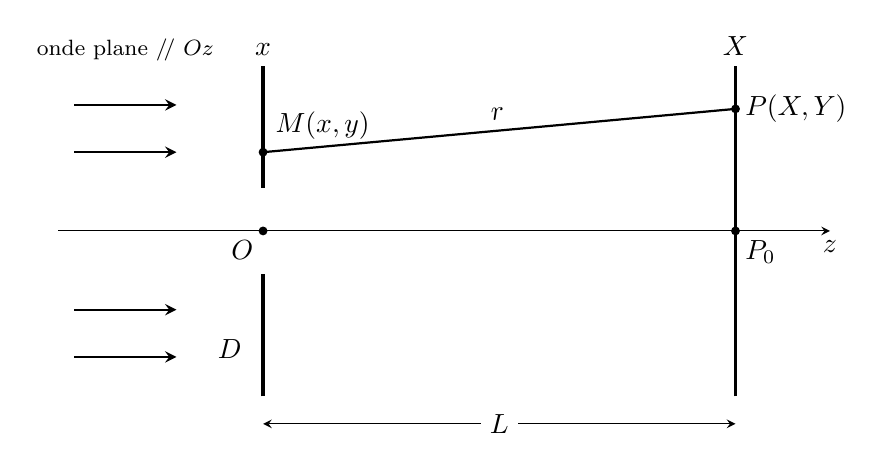
\begin{tikzpicture}[>=stealth, scale=1.0]
    % diffracting screen
    \draw[very thick] (0,-2.1) -- (0,-0.55);
    \draw[very thick] (0,0.55) -- (0,2.1);
    \node[above] at (0,2.1) {$x$};
    \node[left] at (-0.15,-1.5) {$D$};
    % observation plane
    \draw[very thick] (6,-2.1) -- (6,2.1);
    \node[above] at (6,2.1) {$X$};
    % axis
    \draw[->] (-2.6,0) -- (7.2,0) node[below] {$z$};
    % incident plane wave
    \foreach \yy in {-1.6,-1.0,1.0,1.6}{%
      \draw[->,thick] (-2.4,\yy) -- (-1.1,\yy);}
    \node at (-1.75,2.3) {\footnotesize onde plane $/\!/\ Oz$};
    % points
    \fill (0,0) circle (1.6pt) node[below left] {$O$};
    \fill (0,1.0) circle (1.6pt) node[above right=1pt] {$M(x,y)$};
    \fill (6,0) circle (1.6pt) node[below right] {$P_0$};
    \fill (6,1.55) circle (1.6pt) node[right] {$P(X,Y)$};
    \draw[thick] (0,1.0) -- (6,1.55) node[midway,above,sloped] {$r$};
    \draw[<->] (0,-2.45) -- (6,-2.45) node[midway,fill=white] {$L$};
  \end{tikzpicture}
\end{figure}

\begin{definition}[Formule de Fresnel-Kirchhoff (\textit{Fresnel--Kirchhoff formula})]
  Soit $M(x,y)$ un point de l'écran diffractant. Soit $P(X,Y)$ un point dans le
  plan d'observation. L'amplitude complexe de l'onde au point $P$ est
  \[
    U(P) \;=\; \iint\limits_{D}
      \underbrace{U_0(M)}_{\substack{\text{complex amplitude}\\ \text{at } M}}
      \;\;\underbrace{Q(M)}_{\substack{\text{inclination}\\ \text{factor}}}
      \;\;\underbrace{\frac{e^{-i\v{k}\cdot\v{r}}}{r}}_{\text{spherical wave}}\; ds ,
  \]
  (the integral runs over the surface of the diaphragm $D$), où $ds$ est un
  petit élément de surface entourant $M$, $Q(M)$ est un \textbf{facteur
  d'inclinaison} (\textit{inclination factor}) qui dépend de l'angle
  $(\unitv{n}, \vec{MP})$ ($\unitv{n}$ est le vecteur normal à $D$ au point
  $M$), $\v{r} = \vec{MP}$ et $k = 2\pi/\lambda$, avec $\v{k} \,/\!/\, \v{r}$
  (onde sphérique).
\end{definition}

\begin{remark}
  En réalité, cette formule est la formule dite de Fresnel-Kirchhoff dans le cas
  d'un diaphragme plan, obtenue à partir du théorème de Green et de l'équation
  de Helmholtz. Le facteur d'inclinaison (sometimes called « facteur
  d'obliquité ») tient compte du fait qu'en toute rigueur la source ponctuelle
  n'est pas isotrope.
\end{remark}

\subsection{Diffraction par des diaphragmes plans}

Pour un diaphragme plan et si $P$ est très éloigné de la surface $D$ mais proche
de l'axe, on montre que $Q(M)$ est un facteur \emph{constant}. On admettra
qu'il vaut
\[
  Q(M) = \frac{1}{i\lambda},
  \qquad\text{hence}\qquad
  U(P) = \frac{1}{i\lambda}
  \iint\limits_{\substack{\text{surface of the}\\ \text{diaphragm } D}}
  U_0(M)\, \frac{e^{-i\v{k}\cdot\v{r}}}{r}\, ds .
\]
Le facteur $i$ exprime le fait que l'onde secondaire est en quadrature de phase
avec l'onde incidente. Comme ce facteur est commun à toutes les ondes
secondaires, celles-ci restent cohérentes entre elles !

Soit $L$ la distance $OP_0$. On a exactement :
\begin{equation*}
  r = \sqrt{L^2 + (X-x)^2 + (Y-y)^2}
    = L\sqrt{1 + \left(\frac{X-x}{L}\right)^2 + \left(\frac{Y-y}{L}\right)^2}.
\end{equation*}
Selon certaines approximations, cette expression va plus ou moins se simplifier.
C'est ce que l'on va étudier dans la suite de ce chapitre.

\subsubsection{Approximation de Fresnel : diffraction à distance finie}
L'\textbf{approximation de Fresnel} (\textit{Fresnel approximation}) consiste à
considérer l'ouverture diffractante $D$ petite devant $r$ et $L$ ainsi que les
angles petits (étude du phénomène proche de l'axe optique $Oz$).

\paragraph{Première conséquence.} $X - x \ll L$ et $Y - y \ll L$. On peut donc
faire un développement limité de $r$ au premier ordre, avec
$(1+x)^{\alpha} = 1 + \alpha x$ quand $x$ est petit :
\begin{equation*}
  r = L + \frac{(X-x)^2}{2L} + \frac{(Y-y)^2}{2L}.
\end{equation*}

\paragraph{Deuxième conséquence.} Dans l'expression de $U(P)$, $r$ peut être
remplacé par $L$ au dénominateur en considérant que la décroissance de
l'amplitude de chaque onde sphérique est uniforme.

Ainsi, on peut réécrire l'amplitude diffractée dans le cas de la diffraction de
Fresnel :
\begin{equation*}
  U(P) = \frac{1}{i\lambda}\frac{e^{-ikL}}{L}
  \iint\limits_{\substack{\text{surface of the}\\ \text{diaphragm } D}}
  U_0(M)\, e^{-\frac{ik}{2L}\left[(X-x)^2 + (Y-y)^2\right]}\, dx\,dy ,
\end{equation*}
et cette expression peut s'écrire en développant $(X-x)^2$ et $(Y-y)^2$ :
\begin{equation*}
  U(P) = \frac{1}{i\lambda}\frac{e^{-ikL}}{L}\, e^{-\frac{ik}{2L}(X^2+Y^2)}
  \iint\limits_{\substack{\text{surface of the}\\ \text{diaphragm } D}}
  U_0(M)\, e^{-\frac{ik}{2L}(x^2+y^2)}\, e^{+\frac{ik}{L}(Xx+Yy)}\, dx\,dy .
\end{equation*}

Au point $M$, $U_0(M)$ représente l'amplitude du champ transmis par l'écran
diffractant $D$. On peut la réécrire comme l'expression du champ incident
modifiée par $t(x,y)$, une fonction qui représente la \textbf{transmittance} de
l'objet de diffraction et qui est identiquement nulle en dehors de
l'ouverture $D$ :
\begin{equation*}
  U_0(x,y) = E_{\text{incident}}(x,y)\, t(x,y),
  \qquad
  E_{\text{incident}}(x,y) = A_0(x,y)\, e^{-i\phi_0(x,y)} ,
\end{equation*}
avec $A_0$ l'amplitude de l'onde incidente et $\phi_0$ sa phase. On peut alors
étendre les bornes de l'intégrale de $-\infty$ à $+\infty$ puisque $t(x,y)$ est
identiquement nulle en dehors de $D$ :
\begin{equation*}
  U(P) = \frac{1}{i\lambda}\frac{e^{-ikL}}{L}\, e^{-\frac{ik}{2L}(X^2+Y^2)}
  \iint_{-\infty}^{+\infty} E_{\text{incident}}(x,y)\, t(x,y)\,
  e^{-\frac{ik}{2L}(x^2+y^2)}\, e^{+\frac{ik}{L}(Xx+Yy)}\, dx\,dy .
\end{equation*}

\subsubsection{Approximation de Fraunhofer : diffraction à l'infini}
On considère que l'on regarde cette fois le phénomène de diffraction
\emph{à l'infini}, ce que l'on fera à partir de maintenant dans le reste du
module. The \textbf{approximation de Fraunhofer} (\textit{Fraunhofer
approximation}) is the statement that the residual quadratic phase over the
aperture is negligible:
\begin{equation*}
  L \gg \frac{2\pi}{\lambda}\left(\frac{x^2+y^2}{2}\right)
  \qquad\text{so that}\qquad
  e^{-\frac{ik}{2L}(x^2+y^2)} \approx 1 .
\end{equation*}
Ainsi l'amplitude devient, si on écrit la répartition du champ $T$ à l'infini,
quels que soient $X$ et $Y$ :
\begin{equation*}
  U(P) = \frac{1}{i\lambda}
  \underbrace{\frac{e^{-ikL}}{L}\, e^{-\frac{ik}{2L}(X^2+Y^2)}}
             _{\text{phase term} \,\to\, \text{invisible in intensity}}
  \iint_{-\infty}^{+\infty} E_{\text{incident}}(x,y)\, t(x,y)\,
  e^{+\frac{ik}{L}(Xx+Yy)}\, dx\,dy .
\end{equation*}
On constate que l'intégrale prend la forme d'une TF à condition de poser le
changement de variables suivant :
\begin{equation*}
  \boxed{\; u = \frac{X}{\lambda L}, \qquad v = \frac{Y}{\lambda L} \;}
\end{equation*}
$u,v$ seront appelées fréquences spatiales ou angulaires. Soit, après
simplification des termes invisibles en intensité :
\begin{equation*}
  U(u,v) \propto \iint_{-\infty}^{+\infty}
  E_{\text{incident}}(x,y)\, t(x,y)\, e^{-2i\pi(ux+vy)}\, dx\,dy ,
\end{equation*}
et l'on reconnaît alors une transformée de Fourier à deux dimensions --- in the
previous chapter's convention, $\hat{F}(\nu) = \int f(t)e^{-2j\pi\nu t}dt$.

\begin{theorem}[Diffraction de Fraunhofer (\textit{Fraunhofer diffraction})]
  \[
    T(u,v) \;\propto\; TF\!\left[E_{\text{incident}}(x,y)\, t(x,y)\right].
  \]
  Dans l'approximation de Fraunhofer (à l'infini), la diffraction (ou la
  répartition du champ complexe) correspond à la TF du champ après l'écran
  diffractant. La TF s'effectue du domaine de l'espace $(x,y)$ au domaine des
  fréquences spatiales $(u,v)$, les deux espaces duaux de cette TF.
\end{theorem}

\begin{remark}
  The change of variables turns the exponent into $e^{+2i\pi(ux+vy)}$; the
  result above is written with $e^{-2i\pi(ux+vy)}$. This is the convention swap
  noted earlier: decomposing on ondes planes $e^{-j\v{k}\cdot\v{r}}$ makes the
  physical operation an inverse transform, rewritten here as a transformée
  directe so as to keep the convention of chapter 2. For a real transmittance
  nothing observable changes; in general the figure is mirrored through the
  axis (equivalently, orient the axes of the observation plane the other way).
  La convention utilisée pour définir la transformée de Fourier n'est pas
  universelle. Une fois les formules de Fourier écrites, il est impératif de
  continuer à travailler de manière cohérente ; dans le cas d'un autre choix,
  certains facteurs numériques peuvent différer.
\end{remark}

\begin{remark}
  La dépendance en $z$ et $t$ de l'onde incidente n'apparaît pas dans le
  résultat. En réalité, elle existe mais a été omise pour alléger les notations.
  En effet, ne dépendant ni de $x$ ni de $y$, elle intervient en facteur dans
  toutes les équations et n'influence donc pas l'intensité observée (terme de
  phase).
\end{remark}

\subsubsection{Relation entre fréquences spatiales et angles d'inclinaison}
Les variables duales de la TF sont $(x,y)$ côté écran diffractant et $(u,v)$
côté écran d'observation. Si l'on considère, dans l'approximation de Fraunhofer,
que les angles sont petits, on peut écrire :
\begin{equation*}
  \tan\theta_X = \frac{X}{L} \approx \theta_X,
  \qquad
  \tan\theta_Y = \frac{Y}{L} \approx \theta_Y,
\end{equation*}
Si on reprend les expressions du changement de variables, on peut écrire :
\begin{equation*}
  \boxed{\; u = \frac{\theta_X}{\lambda}, \qquad v = \frac{\theta_Y}{\lambda} \;}
\end{equation*}

\begin{conclusion}
  A fréquence spatiale is an \emph{angle divided by a longueur d'onde} ---
  d'où l'expression de « fréquences spatiales ou angulaires ». Plus la
  fréquence spatiale est élevée, plus l'angle est important. La transformée de
  Fourier permet donc de passer de :
  \begin{subpart}
    \item l'espace des positions $(x,y)$ --- \emph{où} la lumière passe après
      l'écran : $t(x,y)$ ;
    \item à l'espace des directions $(u,v) \propto (k_x,k_y) \propto
      (\theta_X,\theta_Y)$ --- \emph{dans quelle direction} va la lumière après
      l'écran à l'infini : $T(u,v)$.
  \end{subpart}
  Ainsi, $T(u,v)$ est le \textbf{spectre angulaire} (\textit{angular
  spectrum}). C'est l'amplitude du champ diffracté en fonction de l'angle (et de
  la longueur d'onde) ; il nous donne donc l'amplitude diffractée dans chaque
  direction :
  \[
    T(u,v) = T\!\left(\frac{X}{\lambda D}, \frac{Y}{\lambda D}\right)
           = T\!\left(\frac{\theta_X}{\lambda}, \frac{\theta_Y}{\lambda}\right).
  \]
  Si on veut connaître la taille de l'image projetée sur un écran, à une
  distance $D$, il suffit de poser le changement de variable pour déduire
  $T(X,Y)$.
\end{conclusion}

La dépendance en $\lambda$ est la raison pour laquelle on observe des irisations
dans les phénomènes de diffraction : lorsque l'on éclaire un écran diffractant
par de la lumière blanche, la position des maxima d'intensité dans la figure de
diffraction dépend de la longueur d'onde.

\begin{example}[Single slit of width $A$]
  A diffracting screen of transmittance $t(x) = \bm{\pi}_A(x)$ --- the porte of
  width $A$ --- lit by an onde plane has spectre angulaire
  \[
    T(u) = T\!\left(\frac{\theta_X}{\lambda}\right) = A\,\frac{\sin \pi u A}{\pi u A},
  \]
  and on an observation screen at distance $D$, after $u = X/\lambda D$,
  \[
    |T(X)|^2 = \left| A\,
      \frac{\sin \pi \frac{X}{\lambda D} A}{\pi \frac{X}{\lambda D} A} \right|^2 .
  \]
  The first zero, i.e.\ the edge of the central lobe, sits at
  $X = \lambda D / A$: the narrower the slit, the more spread out the figure.
\end{example}

\begin{figure}[h!]
  \centering
  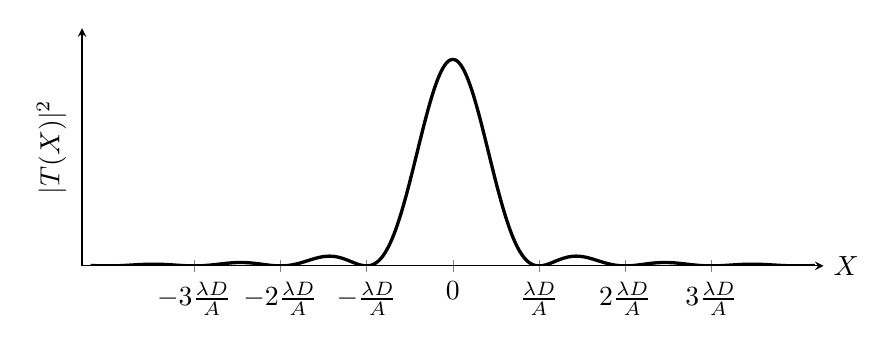
\begin{tikzpicture}
    \begin{axis}[
      width=11cm, height=4.6cm,
      xlabel={$X$}, ylabel={$|T(X)|^2$},
      axis lines=left,
      xmin=-4.3, xmax=4.3, ymin=0, ymax=1.15,
      xtick={-3,-2,-1,0,1,2,3},
      xticklabels={$-3\frac{\lambda D}{A}$,$-2\frac{\lambda D}{A}$,
                   $-\frac{\lambda D}{A}$,$0$,$\frac{\lambda D}{A}$,
                   $2\frac{\lambda D}{A}$,$3\frac{\lambda D}{A}$},
      ytick=\empty,
      every axis x label/.style={at={(current axis.right of origin)},anchor=west},
      ]
      \addplot[very thick,domain=-4.2:4.2,samples=400] {(sin(deg(pi*x))/(pi*x))^2};
    \end{axis}
  \end{tikzpicture}
\end{figure}

\begin{remark}
  Passing from the espace des positions to the espace des directions is not a
  trick reserved for diffraction. Guides à cristaux photoniques : réflexion par
  bande photonique interdite, described in $\v{k}$ space. Mécanique quantique :
  bandes d'énergie exprimées dans le domaine des $\v{k}$ ! Cristal = milliards
  d'atomes : vu le nombre d'atomes, loin des bords, pas de différence entre le
  $n$-ième et le $(n{+}1)$-ième --- l'espace des positions est peu pertinent.
  Connaître les directions de périodicité est plus pertinent.
\end{remark}

\subsubsection{Expression de la transmittance}
Nous avons raisonné jusqu'à présent en supposant que la phase accumulée est la
même en tout point de l'écran diffractant. On peut généraliser en supposant
qu'il y a à la fois des variations d'amplitude et de phase ! Ces variations
peuvent être produites en plaçant dans le plan de l'écran une lame de verre dont
l'absorption et l'épaisseur sont variables :
\begin{subpart}
  \item les variations d'absorption produisent des variations d'amplitude
    $t_D(x,y)$ ;
  \item les variations d'épaisseur ou d'indice de réfraction produisent des
    variations de phase $\phi_D(x,y)$.
\end{subpart}

\begin{definition}[Transmittance]
  D'une manière générale, la transmittance de l'objet devra être identiquement
  nulle en dehors de $D$ et devra représenter ces variations. On écrira donc :
  \[
    t(x,y) = t_D(x,y)\, e^{-i\phi_D(x,y)} .
  \]
\end{definition}

\subsubsection{Expression du champ en sortie de l'écran diffractant}
Dans le cas général, on a vu qu'à l'infini, la répartition du champ correspond à
la TF du produit du champ incident par la transmittance :
\begin{equation*}
  T(u,v) \propto TF\!\left[E_{\text{incident}}(x,y)\, t(x,y)\right]
         \propto TF\!\left[A_0(x,y)\, e^{-i\phi_0(x,y)}\,
                           t_D(x,y)\, e^{-i\phi_D(x,y)}\right],
\end{equation*}
avec $z = 0$ au niveau de l'écran diffractant. Dans le cas d'une onde plane se
propageant parallèlement à l'axe $Oz$, la répartition transverse du champ est
constante. On peut donc écrire le champ incident comme
$E_{\text{incident}}(x,y,z,t) = E_0$ en $z=0$, $t=0$, sans perte de généralité
puisque la TF ne dépend ni de $z$, ni de $t$ !

\begin{corollary}
  \[
    T(u,v) \propto E_0\, TF\!\left[t_D(x,y)\, e^{-i\phi_D(x,y)}\right].
  \]
  Dans le cas d'un écran diffractant éclairé par une onde plane parallèle à
  l'axe $Oz$, l'amplitude complexe de l'onde diffractée à l'infini est
  proportionnelle à la TF de la transmittance de l'écran diffractant.
\end{corollary}

\subsubsection{Où se trouve l'infini ?}
Lorsque $L$ est suffisamment grand, on peut admettre que
\begin{equation*}
  e^{-i\pi\frac{(x^2+y^2)}{\lambda L}} \approx 1 - i\pi\frac{(x^2+y^2)}{\lambda L},
\end{equation*}
et voyons à quelle distance le terme de phase quadratique négligé est 100 fois
plus petit que $1$ (critère arbitraire). On veut :
\begin{equation*}
  \pi\frac{(x^2+y^2)}{\lambda L} < 0.01
  \qquad\Longleftrightarrow\qquad
  L > 100\pi\, \frac{(x^2+y^2)}{\lambda}.
\end{equation*}

\begin{example}
  À $\lambda = 0.6\,\mu\mathrm{m}$ :
  \begin{subpart}
    \item pour une ouverture de $100\,\mu\mathrm{m}$ de diamètre,
      $(x^2+y^2) = r^2 =
      0.25 \cdot 10^{-8}\,\mathrm{m}^2$, soit $z > 1.3\,\mathrm{m}$ ;
    \item pour une ouverture de $1\,\mathrm{cm}$ de diamètre,
      $(x^2+y^2) = r^2 =
      2.5 \cdot 10^{-5}\,\mathrm{m}^2$, soit $z > 13\,000\,\mathrm{m}$.
  \end{subpart}
  Observer de la diffraction sur des ouvertures micrométriques est finalement
  assez simple, l'infini est relativement proche ! Par contre pour un objet
  centimétrique, il est probable qu'à $13\,\mathrm{km}$, il ne reste plus
  beaucoup d'énergie pour observer le phénomène !
\end{example}

\subsection{Diffraction par une lentille}

\subsubsection{Étude intuitive \#1 : la lentille, une transformée de Fourier}
Une source ponctuelle placée au foyer objet d'une lentille génère en sortie une
onde plane déphasée. Que somme-t-on dans le plan focal image ? Des ondes
planes ! Avec $\theta_X = X/f$ et $\theta_x = x/f$,
\begin{equation*}
  T(X) \propto \sum \left[ t_1 \mathbf{1}(x)
     + t_2\, e^{-j\frac{2\pi}{\lambda} X \theta_{x2}} + \cdots \right]
     = \sum \left[ t_1 \mathbf{1}(x)
     + t_2\, e^{-j\frac{2\pi}{\lambda} X \frac{x_2}{f}} + \cdots \right],
\end{equation*}
puis on somme cette fois de façon continue des ondes planes, comme pour la
diffraction à l'infini :
\begin{equation*}
  T\!\left(\frac{X}{\lambda f}\right) = T\!\left(\frac{\theta_X}{\lambda}\right)
  = T(u) \propto \int_{-\infty}^{+\infty} t(x)\,
    e^{-j2\pi x \frac{\theta_X}{\lambda}}\, dx .
\end{equation*}
On retrouve l'expression d'une TF. Les variables duales sont d'un côté l'espace
et de l'autre une variable angulaire comme dans le cas de la diffraction à
l'infini ! $T(u)$ est à nouveau un spectre angulaire !

\subsubsection{Étude intuitive \#2 : la lentille, une transformée de Fourier}
Comme on vient de le voir, tant que l'objet diffractant est petit (inférieur à
$100\,\mu\mathrm{m}$), « l'infini » n'est pas si loin, c'est-à-dire à quelques
mètres. Par contre, pour des objets plus grands, on voit que rapidement,
« l'infini » peut se trouver très loin ! L'observation de la diffraction de
Fraunhofer se trouve donc souvent très difficile. Pour résoudre ce problème, la solution est d'utiliser
une lentille convergente. En effet, une lentille convergente éclairée par une
onde plane (dont les faisceaux se croisent à l'infini) focalise tous les rayons
dans son \textbf{plan focal image} (\textit{image focal plane}) en un point. En
d'autres termes, la lentille ramène dans son plan focal image ce qu'il se passe
à l'infini. Or, en diffraction à l'infini (Fraunhofer), les ondes sphériques
secondaires de Huygens-Fresnel issues de l'écran diffractant sont assimilables à
des ondes planes !

\begin{theorem}[La lentille, une transformée de Fourier]
  Une lentille convergente effectue une transformée de Fourier de la répartition
  du champ complexe depuis son plan focal objet vers son plan focal image. Les
  variables conjuguées sont d'une part, l'espace $(x,y)$ dans le plan focal
  objet et d'autre part, les fréquences spatiales $(u,v)$ dans le plan focal
  image $(X,Y)$, avec
  \[
    u = \frac{X}{\lambda f}, \qquad v = \frac{Y}{\lambda f},
  \]
  où $f$ est la distance focale de la lentille.
\end{theorem}

\begin{figure}[h!]
  \centering
  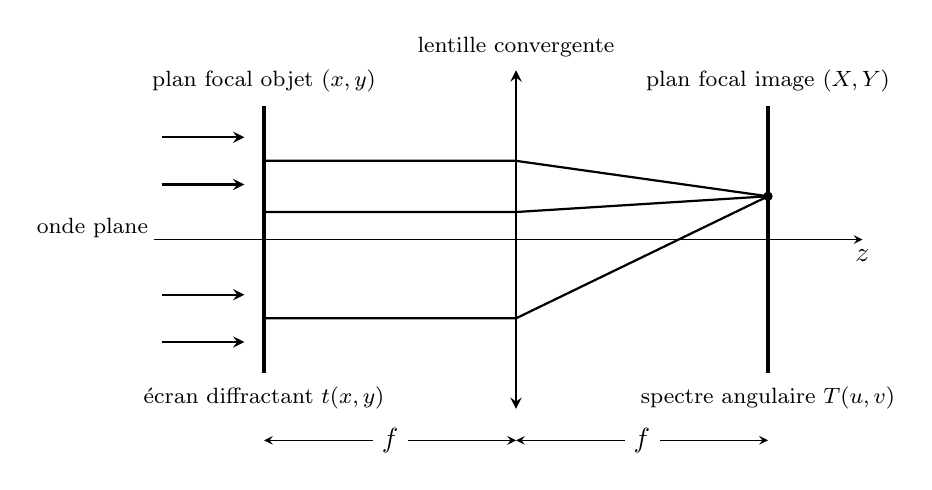
\begin{tikzpicture}[>=stealth]
    % object focal plane
    \draw[very thick] (0,-1.7) -- (0,1.7);
    \node[above] at (0,1.75) {\footnotesize plan focal objet $(x,y)$};
    \node[below] at (0,-1.75) {\footnotesize écran diffractant $t(x,y)$};
    % lens
    \draw[thick] (3.2,-1.85) -- (3.2,1.85);
    \draw[->,thick] (3.2,1.85) -- (3.2,2.15);
    \draw[->,thick] (3.2,-1.85) -- (3.2,-2.15);
    \node[above] at (3.2,2.2) {\footnotesize lentille convergente};
    % image focal plane
    \draw[very thick] (6.4,-1.7) -- (6.4,1.7);
    \node[above] at (6.4,1.75) {\footnotesize plan focal image $(X,Y)$};
    \node[below] at (6.4,-1.75) {\footnotesize spectre angulaire $T(u,v)$};
    % axis
    \draw[->] (-1.4,0) -- (7.6,0) node[below] {$z$};
    % incident plane wave
    \foreach \yy in {-1.3,-0.7,0.7,1.3}{%
      \draw[->,thick] (-1.3,\yy) -- (-0.25,\yy);}
    \node[left] at (-1.35,0.15) {\footnotesize onde plane};
    % rays through lens
    \draw[thick] (0,1.0) -- (3.2,1.0) -- (6.4,0.55);
    \draw[thick] (0,-1.0) -- (3.2,-1.0) -- (6.4,0.55);
    \draw[thick] (0,0.35) -- (3.2,0.35) -- (6.4,0.55);
    \fill (6.4,0.55) circle (1.7pt);
    % distances
    \draw[<->] (0,-2.55) -- (3.2,-2.55) node[midway,fill=white] {$f$};
    \draw[<->] (3.2,-2.55) -- (6.4,-2.55) node[midway,fill=white] {$f$};
  \end{tikzpicture}
\end{figure}

\begin{remark}
  Rigoureusement, la TF exacte est réalisée entre le plan focal \emph{objet} et
  le plan focal \emph{image}. Lorsque l'élément diffractant n'est pas dans le
  plan focal objet, on obtient la même image dans le plan focal image. En fait,
  les calculs laissent apparaître un terme de phase invisible en intensité. This
  can be checked experimentally.
\end{remark}

\subsubsection{La transformée de Fourier par une lentille : calcul explicite}
Cela peut se démontrer de manière rigoureuse en traitant la lentille comme un
masque de phase quadratique ayant un rayon de courbure fonction de la focale.
Write $(\xi,\eta)$ for the transverse coordinates in the plane of the lentille.

\begin{remark}
  The demonstration followed here is written in the \emph{opposite} sign
  convention from the rest of this chapter. The onde incidente is still
  $e^{-ikz}$, but the fonction de transmission is $e^{+i\phi}$ where the
  transmittance above is $t_D e^{-i\phi_D}$, the propagator is $e^{+ikf}$ where
  the one above is $e^{-ikL}$, and the Fresnel kernel is
  $e^{+\frac{ik}{2f}[\cdots]}$ where the one above is
  $e^{-\frac{ik}{2L}[\cdots]}$. The formula applied below is therefore the
  complex conjugate, exponent by exponent, of the expression for $U(P)$ derived
  earlier in this chapter (the prefactor is unchanged, since $1/i = -i$). The
  convention is internally coherent throughout the proof and the result is
  unaffected; this is the same non-universality of the convention already noted
  for the Fraunhofer exponent.
\end{remark}

\paragraph{Fonction de transmission.} The lentille is thin enough that the
lateral translation of the field may be neglected: a small pencil of light
enters at $(\xi,\eta)$ and leaves at $(\xi,\eta)$. If $d(\xi,\eta)$ is the
thickness of glass crossed and $n$ its index, the dephasing on crossing is
$\phi_1(\xi,\eta) = \frac{2\pi n}{\lambda} d(\xi,\eta)$. Between two planes
tangent to the lentille and separated by its maximum thickness $d_0$, the rest
of the path being air,
\begin{equation*}
  \phi(\xi,\eta) = \frac{2\pi n}{\lambda} d(\xi,\eta)
                 + \frac{2\pi}{\lambda}\left(d_0 - d(\xi,\eta)\right)
                 = \frac{2\pi}{\lambda} d_0
                 + \frac{2\pi(n-1)}{\lambda} d(\xi,\eta),
\end{equation*}
so the onde incidente is multiplied by the \textbf{fonction de transmission}
(\textit{transmission function})
\begin{equation*}
  t(\xi,\eta) = e^{i\phi(\xi,\eta)}
              = e^{2i\pi d_0/\lambda}\, e^{2i\pi(n-1)d/\lambda}.
\end{equation*}

\paragraph{L'épaisseur.} Cut the lentille in two along its thickness, with faces
of radii $R_1$ and $R_2$ ($R_2 < 0$):
\begin{equation*}
  d_1 = d_{01} - \left\{ R_1 - \sqrt{R_1^2 - \xi^2 - \eta^2}\right\},
  \qquad
  d_2 = d_{02} - \left\{ -R_2 - \sqrt{R_2^2 - \xi^2 - \eta^2}\right\},
\end{equation*}
whence
\begin{equation*}
  d(\xi,\eta) = d_1 + d_2 = d_0 - \left\{
    R_1 - \sqrt{R_1^2 - \xi^2 - \eta^2} - R_2 - \sqrt{R_2^2 - \xi^2 - \eta^2}
  \right\}.
\end{equation*}
In the paraxial approximation $\xi, \eta \ll R_1, R_2$ and
\begin{equation*}
  R_1 - \sqrt{R_1^2 - \xi^2 - \eta^2}
  = R_1 - R_1\sqrt{1 - \frac{\xi^2}{R_1^2} - \frac{\eta^2}{R_1^2}}
  \simeq \frac{1}{2R_1}\left(\xi^2 + \eta^2\right),
\end{equation*}
so that
\begin{equation*}
  d(\xi,\eta) = d_0 - \frac{1}{2}\left(\xi^2 + \eta^2\right)
                \left[\frac{1}{R_1} - \frac{1}{R_2}\right],
\end{equation*}
and the phase in $t(\xi,\eta)$ becomes
\begin{equation*}
  \phi(\xi,\eta) = \frac{2\pi n}{\lambda} d_0
    - \frac{\pi(n-1)}{\lambda}\left(\xi^2+\eta^2\right)
      \left[\frac{1}{R_1} - \frac{1}{R_2}\right].
\end{equation*}

\paragraph{La distance focale.} This forces the definition
$1/f = (n-1)\left[1/R_1 - 1/R_2\right]$ (the lensmaker's relation), with $f$
indeed the focal length, and
\begin{equation*}
  \boxed{\;
    t(\xi,\eta) = e^{2i\pi n d_0/\lambda}\,
                  e^{-i\pi(\xi^2+\eta^2)/\lambda f}
  \;}
\end{equation*}
The lentille is a pure quadratic phase mask, up to a constant phase.

\begin{example}[Consistency check]
  Let an onde plane $E_i = e^{-ikz}$ be incident on the lentille. The
  transmitted onde is
  \[
    E_t = E_i\, t(\xi,\eta)
        = e^{2i\pi n d_0/\lambda}\,
          e^{-\frac{2i\pi}{\lambda}\left(z + \frac{\xi^2+\eta^2}{2f}\right)},
  \]
  which is an onde sphérique of radius $f$. The lentille transforms an incident
  onde plane into an onde sphérique converging at its image focus --- exactly
  the result used in optique géométrique.
\end{example}

\begin{proof}[Objet contre la lentille, puis objet dans le plan focal objet]
  Consider first a plane object --- a photographic transparency --- placed
  against the lentille, emitting a field $U_i(\xi,\eta)$. Take the pupil function
  equal to $1$, so as not to add the diffraction by the finite aperture of the
  lentille. The field transmitted by the lentille is
  \[
    U_t(\xi,\eta) = U_i(\xi,\eta)\, e^{2i\pi n d_0/\lambda}\,
                    e^{-i\pi(\xi^2+\eta^2)/\lambda f}.
  \]
  Apply the diffraction formula of the approximation de Fresnel over the
  distance $f$ to reach the focal plane:
  \[
    U(x,y) = -\frac{i}{\lambda}\frac{e^{ikf}}{f}
      \iint_{-\infty}^{+\infty}
      e^{\frac{ik}{2f}\left[(x-\xi)^2 + (y-\eta)^2\right]}\,
      U_t(\xi,\eta)\, d\xi\, d\eta .
  \]
  Substituting $U_t$ and using $k/2f = \pi/\lambda f$, the quadratic phase of the
  lentille cancels the $\xi^2 + \eta^2$ produced by expanding the square,
  leaving
  \[
    U(x,y) = -\frac{i}{\lambda}\frac{e^{ikf}}{f}\, e^{2i\pi n d_0/\lambda}\,
      e^{i\pi(x^2+y^2)/\lambda f}
      \iint_{-\infty}^{+\infty} U_i(\xi,\eta)\,
      e^{-\frac{2i\pi}{\lambda f}\left(x\xi + y\eta\right)}\, d\xi\, d\eta .
  \]
  Posing the fréquences spatiales
  \[
    f_x = \frac{\alpha}{\lambda} = \frac{x}{\lambda f},
    \qquad
    f_y = \frac{\beta}{\lambda} = \frac{y}{\lambda f},
  \]
  the integral is the spatial transformée de Fourier $\tilde{U}_i(f_x,f_y)$ of
  $U_i(\xi,\eta)$, and the prefactor $e^{i\pi(x^2+y^2)/\lambda f}$ can be pulled
  out as $e^{i\pi\lambda f (f_x^2 + f_y^2)}$:
  \[
    U(x,y) = \text{Cste}\cdot L(x,y)\cdot \tilde{U}_i(f_x,f_y),
    \qquad
    L(x,y) = e^{i\pi(x^2+y^2)/\lambda f}.
  \]
  The image of $U_i$ in the focal plane is thus its transformée de Fourier
  modified by the \textbf{fonction « loupe »} (\textit{magnifier function})
  $L(x,y)$.\\

  Now move the object out of contact with the lentille and into the \emph{plan
  focal objet}. Let it carry a field $U_0(x_1,y_1)$ with spectre angulaire
  \[
    \tilde{U}_0(f_x,f_y) = \iint_{-\infty}^{+\infty} U_0(x_1,y_1)\,
      e^{-2i\pi\left(f_x x_1 + f_y y_1\right)}\, dx_1\, dy_1 .
  \]
  Propagating over the distance $f$ up to the entrance plane of the lentille, the
  spectre angulaire arriving on the lentille is
  \[
    \tilde{U}_i(f_x,f_y) = \tilde{U}_0(f_x,f_y)\, e^{2i\pi f/\lambda}\,
      e^{-i\pi\lambda f\left(f_x^2 + f_y^2\right)} .
  \]
  Inserting this into the previous relation, the two quadratic phases
  $e^{+i\pi\lambda f(f_x^2+f_y^2)}$ and $e^{-i\pi\lambda f(f_x^2+f_y^2)}$ cancel
  exactly:
  \[
    U(x,y) = -\frac{i}{\lambda}\frac{e^{ikf}}{f}\, e^{2i\pi n d_0/\lambda}\,
       e^{i\pi\lambda f (f_x^2+f_y^2)}\, \tilde{U}_0(f_x,f_y)\,
       e^{2i\pi f/\lambda}\, e^{-i\pi\lambda f(f_x^2+f_y^2)}
  \]
  \[
    \boxed{\;
      U(x,y) = -\frac{i}{\lambda f}\, e^{2ikf}\, e^{2i\pi n d_0/\lambda}\,
               \tilde{U}_0(f_x,f_y)
    \;}
  \]
  The function $L(x,y)$ has disappeared and the image observed in the plan
  focal image is proportional to the transformée de Fourier of the object. \qed
\end{proof}

\begin{conclusion}
  The quadratic phase mask of the lentille always cancels the quadratic phase of
  the Fresnel kernel --- that is what makes the focal-plane field a transformée
  de Fourier at all, object against the lentille included, and it owes nothing
  to where the object sits. What the plan focal objet buys is the
  \emph{second} cancellation: propagation over $f$ from that plane imprints
  $e^{-i\pi\lambda f(f_x^2+f_y^2)}$, exactly the inverse of the residual
  fonction « loupe » $L(x,y)$, so only then is the focal-plane field
  proportional to the bare transform. Placed against the lentille, the object
  still gives its transformée de Fourier, but multiplied by $L(x,y)$ --- a pure
  phase, hence invisible in intensity, which is why the two configurations look
  the same on a screen.
\end{conclusion}

\subsubsection{Méthode de travail : diffraction par une lentille convergente}
Pour résoudre un problème de diffraction par une lentille convergente, la
méthode est toujours la même.
\begin{enumerate}
  \item Dans le plan focal objet, en coordonnées $(x,y)$ : exprimer le champ
    incident ; exprimer la transmittance de l'objet diffractant ; en déduire
    l'expression du champ en sortie de l'écran diffractant.
  \item Dans le plan focal image : calculer l'expression du spectre angulaire
    $T(u,v)$ diffracté dans le plan focal image par transformée de Fourier du
    champ précédent (coordonnées $(u,v)$).
  \item En déduire l'expression du champ diffracté dans le plan focal image, en
    coordonnées spatiales $(X,Y)$ en utilisant le changement de variable
    $u = X/\lambda f$, $v = Y/\lambda f$.
  \item En déduire l'intensité diffractée dans le plan focal image (coordonnées
    $(u,v)$ ou $(X,Y)$).
\end{enumerate}

\subsection{Propriétés générales reliant l'écran diffractant et la figure de diffraction}
Le but de ce paragraphe est de reprendre les propriétés de la TF énoncées dans
le domaine Temps/Fréquence au domaine de la diffraction dans le domaine
Espace/Fréquence spatiale --- with the sign conventions of this chapter.

\subsubsection{TF d'une ouverture carrée}
On peut décomposer la transmittance d'une ouverture carrée de côté $A$ en deux
fonctions à variable séparable :
\begin{equation*}
  t(x,y) = \bm{\pi}_A(x)\, \bm{\pi}_A(y),
\end{equation*}
et le spectre angulaire est la TF de la transmittance puisque l'écran est
éclairé par une onde plane :
\begin{equation*}
  T(u,v) = T\!\left(\frac{\theta_X}{\lambda}\right)
           T\!\left(\frac{\theta_Y}{\lambda}\right)
         \propto \frac{\sin \pi u A}{\pi u A}\,\frac{\sin \pi v A}{\pi v A}.
\end{equation*}
Sur l'écran, on observe l'intensité du signal après le changement de variables,
soit une image de la forme
\begin{equation*}
  |T(X,Y)|^2 \propto
    \left|\frac{\sin \pi \frac{X}{\lambda f}A}{\pi \frac{X}{\lambda f}A}\right|^2
    \left|\frac{\sin \pi \frac{Y}{\lambda f}A}{\pi \frac{Y}{\lambda f}A}\right|^2 ,
\end{equation*}
--- a cross-shaped grid of spots whose central lobe has half-width
$\lambda f / A$.

\subsubsection{TF d'une fente infiniment fine}
On éclaire cette fois une fente infiniment fine et infiniment haute, centrée en
$x=0$. Sa transmittance peut s'exprimer comme $t(x,y) = \delta(x)\mathbf{1}(y)$.
Si on calcule le spectre angulaire diffracté dans le plan focal image, on trouve
cette fois un trait \emph{horizontal} infiniment fin :
\begin{equation*}
  T(u,v) = T\!\left(\frac{\theta_X}{\lambda}\right)
           T\!\left(\frac{\theta_Y}{\lambda}\right)
         \propto \mathbf{1}(u)\,\delta(v),
  \qquad
  |T(X,Y)|^2 \propto |\mathbf{1}(X)|^2 |\delta(Y)|^2 .
\end{equation*}
The pattern is rotated by $90^\circ$ with respect to the object. Ce résultat est
compatible avec la propriété de changement d'échelle below: infinitely narrow
in $x$ gives infinitely wide in $u$, and infinitely wide in $y$ gives
infinitely narrow in $v$. For comparison, a point source centred at the origin
is $t(x,y) = \delta(x)\delta(y)$.

\subsubsection{Dilatation et contraction de l'ouverture du diaphragme}
Si on dilate ou contracte les coordonnées dans l'espace direct, ce qui revient à
multiplier par $a$ et $b$ les dimensions de l'ouverture, on observe inversement
une contraction ou dilatation de l'espace spectral et un changement de
l'amplitude du spectre :
\begin{equation*}
  TF\!\left[t(ax,by)\right] = \frac{1}{|a|}\frac{1}{|b|}\,
    T\!\left(\frac{u}{a}, \frac{v}{b}\right).
\end{equation*}
Plus l'ouverture est petite, plus l'image au foyer image de la lentille est
étalée. The factor $1/|a||b|$ is an energy-conservation factor, as the théorème
de Parseval-Plancherel shows.

\subsubsection{Translation dans son plan du diaphragme limitant la surface d'onde}
Une translation de la fonction $t(x,y)$ dans le plan focal objet se traduit par
la multiplication de l'amplitude de la figure de diffraction par un terme de
phase :
\begin{equation*}
  TF\!\left[t(x-a, y-b)\right] = e^{+2i\pi u a}\, e^{+2i\pi v b}\, T(u,v).
\end{equation*}
Or, en intensité, un terme de phase est invisible puisque son module vaut $1$ !
Donc, \emph{cette translation ne modifiera pas l'image diffractée au plan focal
image}. Réciproquement, un déphasage de l'écran de diffraction provoque un
déplacement de la figure de diffraction. Note that the exponent here carries
$e^{+2i\pi ua}$ where the chapter-2 translation property reads
$TF[f(t-\tau)] = e^{-2i\pi\nu\tau}F[\nu]$: the same inverse-versus-direct
convention swap already noted for the Fraunhofer exponent, and invisible in
intensity either way.

\subsubsection{Succession de transformées de Fourier}
\begin{prop}
  \[
    TF^{-1}\!\left[TF[f(x)]\right] = f(x),
    \qquad
    TF\!\left[TF[f(x)]\right] = f(-x)
    \quad\text{or}\quad
    TF^{-1}\!\left[TF^{-1}[f(x)]\right] = f(-x).
  \]
\end{prop}
Lorsque l'on place une lentille derrière une autre, les deux effectuent la
\emph{même} opération, so two lentilles give $f(-x)$. Conformément à l'optique
géométrique, l'image après deux lentilles est identique à l'originale mais
retournée. Pour simplifier les calculs, on s'affranchira souvent du retournement
de l'image en orientant à l'envers l'axe dans le plan image.

\subsubsection{Distribution peigne de Dirac}
\begin{definition}[Peigne de Dirac]
  Le peigne de Dirac de raison $a$ et son spectre sont :
  \[
    \omega_a(x) = \sum_{n=-\infty}^{+\infty} \delta(x - na),
    \qquad
    TF\!\left[\omega_a(x)\right] = \frac{1}{a}\,\omega_{1/a}(u)
      = \frac{1}{a}\sum_{n=-\infty}^{+\infty} \delta\!\left(u - \frac{n}{a}\right).
  \]
\end{definition}
A comb of pitch $a$ transforms into a comb of pitch $1/a$ and poids $1/a$ --- the
changement d'échelle property again.

\subsection{Convolution et multiplication}

\begin{definition}[Produit de convolution (\textit{convolution product})]
  \[
    h(x) = (f * f')(x) = \int_{-\infty}^{+\infty} f(x')\, f'(x-x')\, dx' .
  \]
\end{definition}

Le produit de convolution est essentiel en physique car il apparaît dès que l'on
effectue une \emph{mesure} mais il peut être dur à calculer.

\begin{theorem}[Théorème de convolution (\textit{convolution theorem})]
  La TF d'un produit de convolution $(*)$ de deux fonctions est égale au produit
  simple $(\times)$ des TF et réciproquement :
  \[
    (f * g)(x)
    \quad\stackrel{TF}{\longleftrightarrow}\quad
    \hat{F}(u) \times \hat{G}(u).
  \]
\end{theorem}

On voit qu'un calcul de convolution qui peut être très complexe peut se
transformer en un produit bien plus simple en passant par transformée de Fourier
dans le domaine dual.

\begin{remark}
  Attention au cas de la TF à deux dimensions : convoluer deux fonctions de
  variables \emph{différentes} n'a aucun sens physique, c'est donc interdit. À
  deux dimensions, dans le cas de fonctions à variables séparables, une
  multiplication reste donc une multiplication ! On écrira :
  \[
    f(x) \times g(y)
    \quad\stackrel{TF}{\longleftrightarrow}\quad
    \hat{F}(u) \times \hat{G}(v),
  \]
  which is immediate from
  $TF[f(x)g(y)] = \iint f(x)g(y) e^{-2j\pi(ux+vy)}dx\,dy
   = \int f(x)e^{-2j\pi ux}dx \int g(y)e^{-2j\pi vy}dy$.
\end{remark}

\begin{prop}[Quelques propriétés du produit de convolution]
  \begin{subpart}
    \item commutatif : $(f*g)(x) = (g*f)(x)$ ;
    \item associatif : $\left(f*(g*h)\right)(x) = \left((f*g)*h\right)(x)$ ;
    \item distributif : $\left([a\cdot f + b\cdot g] * h\right)(x)
      = a\cdot(f*h)(x) + b\cdot(g*h)(x)$.
  \end{subpart}
\end{prop}

\subsubsection{Convolution d'une fonction avec un Dirac ou un peigne de Dirac}
D'après ce qui précède (théorème de convolution), on peut écrire :
\begin{equation*}
  TF\!\left[(f*\delta)(x)\right] = TF[f(x)]\, TF[\delta(x)] = TF[f(x)],
  \qquad\text{hence}\qquad
  (f*\delta)(x) = \int f(x')\delta(x-x')dx' = f(x).
\end{equation*}
\emph{Le Dirac est l'élément neutre de la convolution !} Plus intéressant encore,
la convolution d'une fonction avec un Dirac décentré donne, en effectuant un
changement de variable adéquat :
\begin{equation*}
  \boxed{\; f(x) * \delta(x-a) = f(x-a) \;}
\end{equation*}
La convolution d'une fonction avec un Dirac décentré redonne la même fonction
mais centrée à la position du Dirac. Cette opération permet donc de
\textbf{translater} une fonction. On constate que, bien que le Dirac n'ait pas
de réalité physique, sa convolution avec une fonction donne une fonction, le
résultat a donc une réalité physique.

La convolution ainsi que la TF étant distributives, on obtient naturellement :
\begin{equation*}
  f(x) * \omega_a(x) = f(x) * \sum_{n=-\infty}^{+\infty}\delta(x - na)
                     = \sum_{n=-\infty}^{+\infty} f(x - na) .
\end{equation*}
La convolution d'une fonction avec une somme de Diracs permet donc de
\textbf{périodiser} une fonction. C'est comme cela que nous représenterons les
fonctions périodiques, avec $f(x)$ qui représentera le motif élémentaire. Cela
facilitera grandement les calculs.

\subsubsection{Multiplication d'une fonction avec un Dirac}
\begin{equation*}
  \boxed{\; f(x) \times \delta(x-a) = f(a)\,\delta(x-a) \;}
\end{equation*}
L'intérêt de cette propriété est de simplifier les calculs en transformant une
fonction en une constante, la valeur de la fonction à la position du Dirac.
Cette constante modifie « le poids » du Dirac. Attention, il est indispensable
de ne pas oublier le Dirac sans quoi le résultat est complètement faux !

\begin{conclusion}[Convolution ou multiplication ?]
  Pas de hasard ! On utilisera la \textbf{multiplication} pour modifier les
  amplitudes d'une fonction ; on utilisera la \textbf{convolution avec un Dirac}
  pour translater une fonction.
\end{conclusion}

\begin{example}[The monochromator]
  A monochromator disperses the spectrum in space and scans it with a moving slit
  in front of a detector. The measured signal is the real spectrum convolved with
  the sliding window, which is a porte:
  \[
    S_{\text{mesuré}}(\lambda) = \int_{-\infty}^{+\infty}
      S_{\text{réel}}(x')\, \underbrace{\bm{\pi}(\lambda - x')}
      _{\text{fenêtre glissante} \,=\, \text{porte}}\, dx' .
  \]
  When the window is narrow, $\bm{\pi}_\varepsilon \to \delta$ and the measured
  spectrum is the real one; when it is broad, the fine structure is smoothed away.
  Every instrument convolves what it measures by its own \textit{fonction
  d'appareil}.
\end{example}

\begin{example}[Listening to a sound]
  In the frequency domain, the spectrum $S(\nu)$ of a sound is \emph{multiplied}
  by the filtre passe-bande of the ear, of bande passante $BP$. In the time
  domain the same operation is a convolution of $s(t) = TF[S(\nu)]$ by the instrument
  function $TF[\text{filtre de l'oreille}]$, whose width is the integration time
  $\Delta\tau \propto 1/BP$ of the detector. A sound too high in pitch oscillates
  faster than $\Delta\tau$, is averaged out, and is not heard.
\end{example}

\subsection{Lien entre variations d'intensité dans une image et fréquences spatiales}
Une fréquence spatiale peut être vue comme un angle qui dépend de la longueur
d'onde. En d'autres termes, dans le plan focal image d'une lentille, plus les
fréquences spatiales sont élevées, plus l'énergie se retrouve répartie loin de
l'axe optique. Plus les fréquences spatiales sont basses, plus l'énergie se
retrouve proche de l'axe optique.

\subsubsection{Signification de $T(0,0)$}
Si on reprend l'expression de la TF en $u = v = 0$, on obtient :
\begin{equation*}
  T(u,v)\big|_{u=v=0} \propto \iint_{-\infty}^{+\infty}
    E_{\text{incident}}(x,y)\, t(x,y)\, e^{-2i\pi(0x+0y)}\, dx\, dy
  \propto \iint_{-\infty}^{+\infty} E_{\text{incident}}(x,y)\, t(x,y)\, dx\, dy ,
\end{equation*}
c'est bien la \emph{moyenne} de l'onde dans le plan focal objet --- the centre
of the figure de diffraction carries the continuous background of the image.

\subsubsection{Signification de $T(u,v)$ pour $u,v$ différents de 0}
Prenons un \textbf{réseau sinusoïdal} (\textit{sinusoidal grating}) de pas $a$,
de dimension infinie dans les deux directions :
\begin{equation*}
  t_{\substack{\text{réseau}\\ \text{infini}}}(x,y)
    = \left(\frac{1}{2} + \cos\left(\frac{2\pi x}{a}\right)\right)\mathbf{1}(y),
\end{equation*}
avec $\mathbf{1}(y)$ la fonction qui vaut $1$ quel que soit $y$. Dans le plan
focal image de la lentille, on observe la TF de l'écran diffractant :
\begin{equation*}
  T_{\substack{\text{réseau}\\ \text{infini}}}(u,v)
    = \frac{1}{2}\left(\delta(u)
      + \delta\!\left(u + \frac{1}{a}\right)
      + \delta\!\left(u - \frac{1}{a}\right)\right)\delta(v).
\end{equation*}

\begin{remark}
  La fonction $\mathbf{1}(y)$ semble ne servir à rien. Il est vrai que ne pas
  l'écrire n'est pas faux. Par contre, l'omettre, c'est très souvent oublier
  d'en faire la TF, ce qui modifie notablement le résultat car
  $TF[\mathbf{1}(y)] = \delta(v)$.
\end{remark}

On observe donc deux taches au côté de la tache centrale.
\begin{subpart}
  \item La tache centrale $\delta(u)$ porte l'information sur le fond continu
    --- la valeur moyenne --- de l'écran diffractant.
  \item Les deux taches adjacentes $\delta(u \pm 1/a)$ sont la signature
    spectrale de la variation d'amplitude sinusoïdale de l'écran de diffraction.
  \item L'extension suivant $Y$ est nulle, $\delta(v)$, puisqu'elle était
    infinie, $\mathbf{1}(y)$, dans l'écran diffractant.
\end{subpart}

On peut tronquer mathématiquement le réseau de dimension infinie en le
multipliant par une porte de largeur adéquate $A$ :
\begin{equation*}
  t_{\substack{\text{réseau}\\ \text{tronqué}}}(x,y)
    = \bm{\pi}\!\left(\frac{x}{A}\right) \times
      t_{\substack{\text{réseau}\\ \text{infini}}}(x,y),
\end{equation*}
and by the théorème de convolution the multiplication in direct space becomes a
convolution in the spectral space:
\begin{align*}
  T_{\substack{\text{réseau}\\ \text{tronqué}}}(u,v)
  &= TF\!\left[\bm{\pi}\!\left(\frac{x}{A}\right)\right] *
     T_{\substack{\text{réseau}\\ \text{infini}}}(u,v) \\
  &= \frac{1}{2} A \frac{\sin \pi u A}{\pi u A} *
     \left(\delta(u) + \delta\!\left(u+\frac{1}{a}\right)
     + \delta\!\left(u-\frac{1}{a}\right)\right)\delta(v) \\
  &\propto \left(\frac{\sin \pi u A}{\pi u A}
     + \frac{\sin \pi \left(u+\frac{1}{a}\right)A}{\pi\left(u+\frac{1}{a}\right)A}
     + \frac{\sin \pi \left(u-\frac{1}{a}\right)A}{\pi\left(u-\frac{1}{a}\right)A}
     \right)\delta(v).
\end{align*}
La figure de diffraction est la même que pour le réseau infini mais les pics sont
remplacés par des taches de diffraction (ici des sinus cardinaux) car le réseau
est tronqué, de largeur $A$.

\begin{figure}[h!]
  \centering
  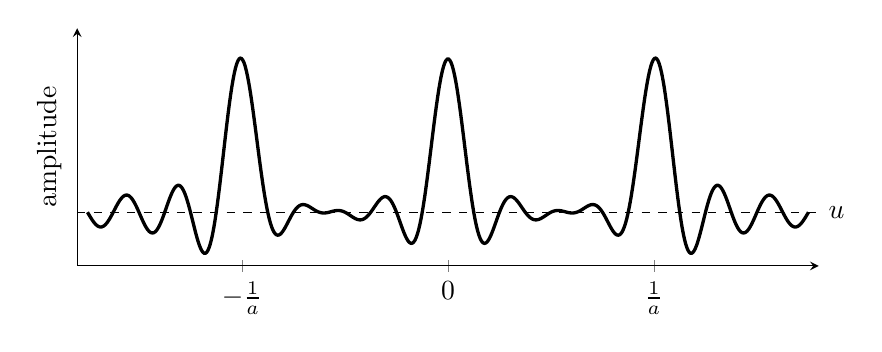
\begin{tikzpicture}
    \begin{axis}[
      width=11cm, height=4.6cm,
      xlabel={$u$}, ylabel={amplitude},
      axis lines=left,
      xmin=-3.6, xmax=3.6, ymin=-0.35, ymax=1.2,
      xtick={-2,0,2},
      xticklabels={$-\frac{1}{a}$,$0$,$\frac{1}{a}$},
      ytick=\empty,
      every axis x label/.style={at={(current axis.right of origin)},anchor=west},
      ]
      \addplot[very thick,domain=-3.5:3.5,samples=600]
        {sin(deg(pi*4*x))/(pi*4*x)
         + sin(deg(pi*4*(x+2)))/(pi*4*(x+2))
         + sin(deg(pi*4*(x-2)))/(pi*4*(x-2))};
      \draw[dashed] (axis cs:-3.6,0) -- (axis cs:3.6,0);
    \end{axis}
  \end{tikzpicture}
\end{figure}

La position des deux pics adjacents dépend de la période du réseau sinusoïdal.
En accord avec la propriété de contraction/dilatation :
\begin{subpart}
  \item plus la variation d'amplitude de l'écran diffractant est lente (large
    period), plus la fréquence est basse et la position des pics adjacents est
    proche de l'axe optique ($X$ et $Y$ faibles) ;
  \item plus la variation d'amplitude de l'écran diffractant est rapide (small
    period), plus la fréquence est élevée et la position du pic est éloignée de
    l'axe optique ($X$ et $Y$ élevés) ;
  \item l'information spectrale concernant le fond continu ou la valeur moyenne
    d'une image sera elle représentée au centre, $u = v = X = Y = 0$.
\end{subpart}

\begin{conclusion}
  Pour une image quelconque :
  \begin{subpart}
    \item les variations rapides --- les contours d'un objet, les détails, les
      rayures --- seront représentées sur l'écran de diffraction par de
      l'énergie lumineuse \emph{loin} de l'axe optique ;
    \item les variations lentes, les couleurs uniformes et la valeur moyenne de
      l'image seront représentées par de l'énergie lumineuse \emph{proche} de
      l'axe.
  \end{subpart}
  La notion de fréquence spatiale représente donc en quelque sorte le nombre de
  variations par unité de longueur. Pour un réseau, on parle de nombre de traits
  par millimètre. La figure de diffraction nous informe donc sur les
  périodicités présentes dans l'image !
\end{conclusion}

\subsection{Traitement des images}
Le filtrage est une notion finalement assez connue par bon nombre de personnes
pour peu qu'elles aient eu une fois dans leur vie un égaliseur de chaîne HIFI où
tout naturellement nous atténuons telle ou telle fréquence comme les aigus ou
les graves. Seul l'étourdi n'aura pas remarqué qu'il applique alors des
\textbf{filtres passe-bande} (\textit{band-pass filters}) laissant passer ou
coupant certaines bandes de fréquence. Avec une
lentille, nous pouvons isoler \emph{dans l'espace} telle ou telle fréquence
spatiale. Il est alors facile de comprendre que dans le plan focal image d'une
lentille, il est possible de « couper » certaines fréquences par un simple cache
pour obturer la lumière. Une lentille supplémentaire permet alors de repasser
dans l'espace principal et reconstituer l'image filtrée.

\begin{definition}[Montage 4f]
  Le \textbf{montage 4f} (\textit{4f setup}), dit « à double diffraction », est
  composé de deux lentilles placées sur le même axe optique, dont le foyer image
  de la première coïncide avec le foyer objet de la seconde. C'est ce que l'on
  appelle un \textbf{système afocal} (\textit{afocal system}). La diapositive
  dans le plan focal objet est éclairée par une onde plane. The common focal
  plane is the \textbf{plan de Fourier} (\textit{Fourier plane}), que l'on peut
  également appeler \textbf{plan de filtrage} (\textit{filtering plane}).
\end{definition}

\begin{figure}[h!]
  \centering
  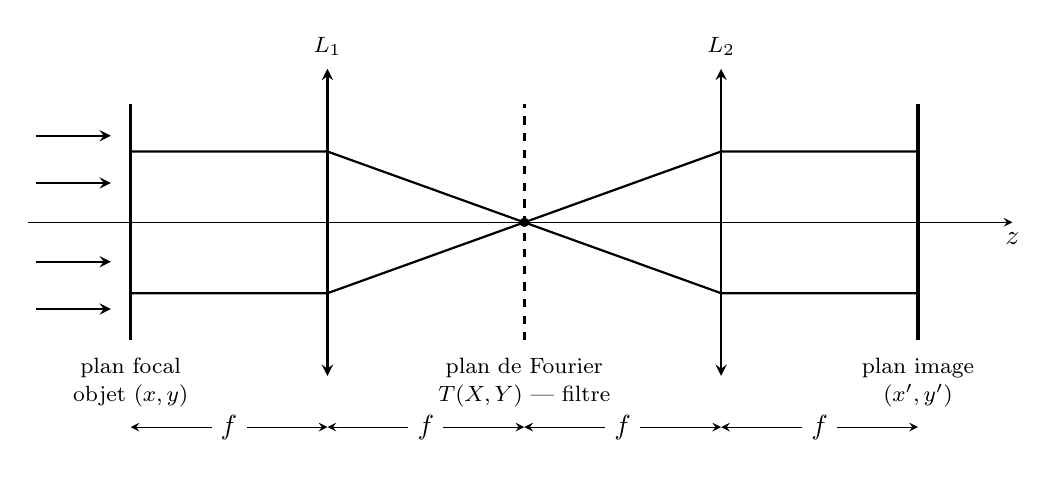
\begin{tikzpicture}[>=stealth]
    \draw[->] (-1.3,0) -- (11.2,0) node[below] {$z$};
    % object plane
    \draw[very thick] (0,-1.5) -- (0,1.5);
    \node[align=center,below] at (0,-1.6)
      {\footnotesize plan focal\\[-2pt] \footnotesize objet $(x,y)$};
    % lens 1
    \draw[thick] (2.5,-1.65) -- (2.5,1.65);
    \draw[->,thick] (2.5,1.65) -- (2.5,1.95);
    \draw[->,thick] (2.5,-1.65) -- (2.5,-1.95);
    \node[above] at (2.5,2.0) {\footnotesize $L_1$};
    % Fourier plane
    \draw[very thick,dashed] (5,-1.5) -- (5,1.5);
    \node[align=center,below] at (5,-1.6)
      {\footnotesize plan de Fourier\\[-2pt] \footnotesize $T(X,Y)$ --- filtre};
    % lens 2
    \draw[thick] (7.5,-1.65) -- (7.5,1.65);
    \draw[->,thick] (7.5,1.65) -- (7.5,1.95);
    \draw[->,thick] (7.5,-1.65) -- (7.5,-1.95);
    \node[above] at (7.5,2.0) {\footnotesize $L_2$};
    % image plane
    \draw[very thick] (10,-1.5) -- (10,1.5);
    \node[align=center,below] at (10,-1.6)
      {\footnotesize plan image\\[-2pt] \footnotesize $(x',y')$};
    % rays
    \draw[thick] (0,0.9) -- (2.5,0.9) -- (5,0.0) -- (7.5,-0.9) -- (10,-0.9);
    \draw[thick] (0,-0.9) -- (2.5,-0.9) -- (5,0.0) -- (7.5,0.9) -- (10,0.9);
    \fill (5,0) circle (1.7pt);
    % plane wave
    \foreach \yy in {-1.1,-0.5,0.5,1.1}{%
      \draw[->,thick] (-1.2,\yy) -- (-0.25,\yy);}
    % distances
    \foreach \xa/\xb in {0/2.5, 2.5/5, 5/7.5, 7.5/10}{%
      \draw[<->] (\xa,-2.6) -- (\xb,-2.6) node[midway,fill=white] {$f$};}
  \end{tikzpicture}
\end{figure}

Conformément à l'optique géométrique, sans filtrage, on retrouve l'image
identique mais inversée. C'est aussi conforme à l'optique de Fourier puisqu'après
deux TF successives :
\begin{equation*}
  TF\!\left[TF[f(x,y)]\right] = f(-x,-y).
\end{equation*}

Dans le plan de Fourier, on peut alors insérer différents masques ou filtres.
\begin{subpart}
  \item Le \textbf{filtre passe-bas} (\textit{low-pass filter}) --- une ouverture
    circulaire --- coupe les hautes fréquences. On l'a vu, ces fréquences portent
    l'information sur les détails d'une image, les variations rapides
    d'intensité. L'image filtrée se retrouvera donc \emph{floutée}.
  \item Le \textbf{filtre passe-haut} (\textit{high-pass filter}) --- une
    pastille absorbante (on the axis) --- fait l'inverse du passe-bas. Il coupe
    le fond continu d'une image et toutes les variations lentes d'intensité. Il
    ne restera donc dans l'image filtrée que les \emph{contours} des formes.
  \item Between the two sits the filtre passe-bande, an annulus.
\end{subpart}

\begin{remark}
  Two further applications: le \textit{détramage} de photo --- removing the
  printing screen of a photograph, whose regular raster shows up as isolated
  spots in the plan de Fourier that can simply be blocked --- and l'extraction
  des variations de phase invisibles à l'œil nu, a phase object being invisible
  in intensity until its spectrum is filtered.
\end{remark}

\begin{conclusion}
  The whole chapter reduces to one operation and one change of variables. At
  infinity --- or, equivalently, in the plan focal image of a lentille
  convergente --- the diffracted amplitude complexe is the transformée de
  Fourier of the field leaving the diffracting screen,
  \[
    T(u,v) \propto TF\!\left[E_{\text{incident}}(x,y)\, t(x,y)\right],
    \qquad
    u = \frac{X}{\lambda f} = \frac{\theta_X}{\lambda},
    \qquad
    v = \frac{Y}{\lambda f} = \frac{\theta_Y}{\lambda}.
  \]
  Everything else --- the sinc of a slit, the inverse scaling of the pattern with
  the aperture, the invisibility of a translation, the periodisation by a
  peigne de Dirac, low-pass and high-pass filtering --- is a property of that
  transform read in optical language.
\end{conclusion}
